\documentclass[landscape]{article}
\usepackage{tikz}
\usetikzlibrary{trees, positioning}

\begin{document}

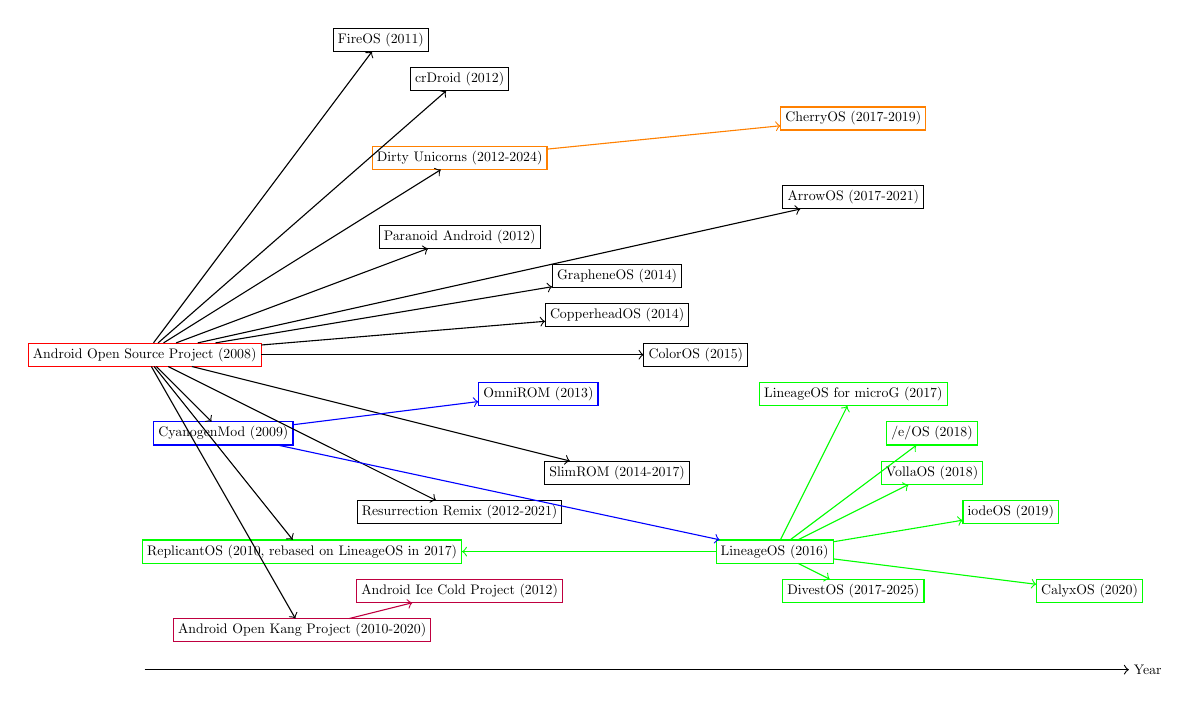
\begin{tikzpicture}[node distance=2cm, scale=0.5, transform shape]
  % Draw the year line
  \draw [->] (0,0) -- (25,0) node [right] {Year};
  
  % Draw the year labels
%   \foreach \x in {2008, 2009, 2010, 2011, 2012, 2013, 2014, 2015, 2016, 2017, 2018, 2019, 2020, 2021, 2022, 2023, 2024, 2025}
%   \draw (\x-2008,0) -- (\x-2008,-0.1) node [below] {\x};
  
  % Create the nodes
  \node (android) [rectangle, draw=red] at (0,8) {Android Open Source Project (2008)};
  \node (fireos) [rectangle, draw] at (6,16) {FireOS (2011)};
  \node (crdroid) [rectangle, draw] at (8,15) {crDroid (2012)};

  \node (dirtyunicorns) [rectangle, draw=orange] at (8,13) {Dirty Unicorns (2012-2024)};
  \node (cherryos) [rectangle, draw=orange] at (18,14) {CherryOS (2017-2019)};

  \node (paranoidandroid) [rectangle, draw] at (8,11) {Paranoid Android (2012)};
  \node (coloros) [rectangle, draw] at (14,8) {ColorOS (2015)};
  \node (copperheados) [rectangle, draw] at (12,9) {CopperheadOS (2014)};
  \node (arrowos) [rectangle, draw] at (18,12) {ArrowOS (2017-2021)};

  \node (cyanogenmod) [rectangle, draw=blue] at (2,6) {CyanogenMod (2009)};
  \node (omnirom) [rectangle, draw=blue] at (10,7) {OmniROM (2013)};
  \node (lineageos) [rectangle, draw=green] at (16,3) {LineageOS (2016)};

  \node (lineageos microg) [rectangle, draw=green] at (18,7) {LineageOS for microG (2017)};
  \node (eos) [rectangle, draw=green] at (20,6){/e/OS (2018)};
  \node (vollaos) [rectangle, draw=green] at (20,5) {VollaOS (2018)};
  \node (iodeos) [rectangle, draw=green] at (22,4) {iodeOS (2019)};
  \node (divestos) [rectangle, draw=green] at (18,2) {DivestOS (2017-2025)};
  \node (calyxos) [rectangle, draw=green] at (24,2) {CalyxOS (2020)};
  \node (replicantos) [rectangle, draw=green] at (4,3) {ReplicantOS (2010, rebased on LineageOS in 2017)};

  \node (aokp) [rectangle, draw=purple] at (4,1) {Android Open Kang Project (2010-2020)};
  \node (androidicecold) [rectangle, draw=purple] at (8,2) {Android Ice Cold Project (2012)};

  \node (resurrectionremix) [rectangle, draw] at (8,4) {Resurrection Remix (2012-2021)};
  \node (grapheneos) [rectangle, draw] at (12,10) {GrapheneOS (2014)};
  \node (slimrom) [rectangle, draw] at (12,5) {SlimROM (2014-2017)};
  
  \draw [->] (android) -- (replicantos);
  \draw [->] (android) -- (fireos);
  \draw [->] (android) -- (grapheneos);
  \draw [->] (android) -- (slimrom);
  \draw [->] (android) -- (resurrectionremix);
  \draw [->] (android) -- (crdroid);
  \draw [->] (android) -- (paranoidandroid);
  \draw [->] (android) -- (copperheados);
  \draw [->] (android) -- (coloros);
  \draw [->] (android) -- (arrowos);

  \draw [->] (android) -- (dirtyunicorns);
  \draw [->, draw=orange] (dirtyunicorns) -- (cherryos);

  \draw [->] (android) -- (aokp);
  \draw [->, draw=purple] (aokp) -- (androidicecold);

  \draw [->] (android) -- (cyanogenmod);
  \draw [->, draw=blue] (cyanogenmod) -- (omnirom);
  \draw [->, draw=blue] (cyanogenmod) -- (lineageos);

  \draw [->, draw=green] (lineageos) -- (divestos);
  \draw [->, draw=green] (lineageos) -- (lineageos microg);
  \draw [->, draw=green] (lineageos) -- (replicantos);
  \draw [->, draw=green] (lineageos) -- (vollaos);
  \draw [->, draw=green] (lineageos) -- (eos);
  \draw [->, draw=green] (lineageos) -- (iodeos);
  \draw [->, draw=green] (lineageos) -- (calyxos);
\end{tikzpicture}

\end{document}